\documentclass[12pt,a4paper,english
% ,twoside,openright
]{tutthesis}
%\documentclass[12pt,a4paper,finnish]{tutthesis}

% Note that you must choose either Finnish or English here and there in this
% file.
% Other options for document class
  % ,twoside,openright   % If printing on both sides (>80 pages)
  % ,twocolumn           % Can be used in lab reports, not in theses

% Ensure the correct Pdf size (not needed in all environments)
\special{papersize=210mm,297mm}


% LaTeX file for BSC/MSc theses and lab reports.
% Requires the class file (=template) tutthesis.cls and figure files,
% either tut-logo, exampleFig (as pdf or eps) and example_code.c
% Author: Sami Paavilainen (2006)
% Modified: Heikki Huttunen (heikki.huttunen@tut.fi) 31.7.2012.
%           Erno Salminen, @tut.fi, 2014-08-15
%             - added text snippets from the writing guide
%             - added lots of comments: both tips and alternative styles
%             - added an example table
%             - and so on...

%
% Define your basic information
%
\author{Jaakko Pasanen}
\title{Natural Language Syntactic Parsing with Deep Learning} % primary title (for front page)
\titleB{Luonnollisen kielen syntaksin parsiminen syväoppimisella}     % translated title for abstract
\thesistype{Master of Science thesis} % or Bachelor of Science, Laboratory Report... 
\examiner{Ari Visa} % without title Prof., Dr., MSc or such

% Put your thesis' main language last
% http://mirrors.ctan.org/macros/latex/required/babel/base/babel.pdf
\usepackage[finnish, main=english]{babel}

% http://www.ctan.org/pkg/biblatex
\usepackage[
  style=authoryear,
  maxcitenames=2,
  backend=biber,
  firstinits=true
]{biblatex}
\bibliography{thesis_refs.bib}
%% Note that option style=numeric works as well
\usepackage{fontspec}
\usepackage{amsfonts}


% You can also add your own commands
\newcommand\todo[1]{{\color{red}TODO: #1}} % Remark text in braces appears in red
\newcommand{\angs}{\textsl{\AA}}              % , e.g. slanted symbol for Ångstöm

% Preparatory content ends here


\pagenumbering{roman} % was: {Roman}
\pagestyle{headings}
\begin{document}

% Special trick so that internal macros (denoted with @ in their name)
% can be used outside the cls file (e.g. \@author)
\makeatletter

%
% Create the title page.
% First the logo. Check its language.
\thispagestyle{empty}
\vspace*{-.5cm}\noindent

\includegraphics[width=8cm]{tty_tut_logo}   % Bilingual logo

% Then lay out the author, title and type to the center of page.
\vspace{6.8cm}
\maketitle
\vspace{6.7cm} % -> 6.7cm if thesis title needs two lines

% Last some additional info to the bottom-right corner
\begin{flushright}  
  \begin{minipage}[c]{6.8cm}
    \begin{spacing}{1.0}
      %\textsf{Tarkastaja: Prof. \@examiner}\\
      %\textsf{Tarkastaja ja aihe hyväksytty}\\ 
      %\textsf{xxxxxxx tiedekuntaneuvoston}\\
      %\textsf{kokouksessa dd.mm.yyyy}\\
      \textsf{Examiner: Prof. \@examiner}\\
      \textsf{Examiner and topic approved by the}\\ 
      \textsf{Faculty Council of the Faculty of}\\
      \textsf{Engineering Sciences}\\
      \textsf{on 31st December 2017}\\
    \end{spacing}
  \end{minipage}
\end{flushright}

% Leave the backside of title page empty in twoside mode
\if@twoside
\clearpage
\fi

%
% Use Roman numbering I,II,III... for the first pages (abstract, TOC,
% termlist etc)
\pagenumbering{Roman} 
\setcounter{page}{0} % Start numbering from zero because command 'chapter*' does page break

% Some fields in abstract are automated, namely those with \@ (author,
% title in the main language, thesis type, examiner).
\chapter*{Abstract}

\begin{spacing}{1.0}
         {\bf \textsf{\MakeUppercase{\@author}}}: \@title\\   % use \@titleB when thesis is in Finnish
         \textsf{Tampere University of Technology}\\
         \textsf{\@thesistype, xx pages, x Appendix pages} \\
         \textsf{December 2016}\\
         \textsf{Master's Degree Programme in Automation Technology}\\
         \textsf{Major: Learning and Intelligent Systems}\\
         \textsf{Examiner: Prof. \@examiner}\\ % 
         \textsf{Keywords: Hype}\\
\end{spacing}


The abstract is a concise 1-page description of the work: what was the
problem, what was done, and what are the results. Do not include
charts or tables in the abstract.

Put the abstract in the primary language of your thesis first and then
the translation (when that is needed).


% Foreign students do not need Fininsh abstract (tiivistelmä). Move
% this before English abstract if thesis is in Finnish. Move also the
% otherlanguage command to the English abstract (if needed).

\begin{otherlanguage}{finnish} %  Following text in in 2nd language
\chapter*{Tiivistelmä} % Asterisk * turns numbering off

\begin{spacing}{1.0}
         {\bf \textsf{\MakeUppercase{\@author}}}: \@titleB\\  % or use \@title when thesis is in Finnish
         \textsf{Tampereen teknillinen yliopisto}\\
         \textsf{Diplomityö, xx sivua, x liitesivua}\\ %
         \textsf{Joulukuu 2016}\\
         \textsf{Automaatiotekniikan koulutusohjelma}\\
         \textsf{Pääaine: Oppivat ja älykkäät järjestelmät}\\
         \textsf{Tarkastajat:  Prof. \@examiner}\\ % automated, if just 1 examiner
         \textsf{Avainsanat: Hype}\\
\end{spacing}

The abstract in Finnish. Foreign students do not need this page.

Suomenkieliseen diplomityöhön kirjoitetaan tiivistelmä sekä suomeksi
että englanniksi.

Kandidaatintyön tiivistelmä kirjoitetaan ainoastaan kerran, samalla
kielellä kuin työ. Kuitenkin myös suomenkielisillä kandidaatintöillä
pitää olla englanninkielinen otsikko arkistointia varten.

\end{otherlanguage} % End on 2nd language part


\chapter*{Preface}

This document template conforms to Guide to Writing a Thesis at
Tampere University of Technology (2014) and is based on the previous
template. The main purpose is to show how the theses are formatted
using LaTeX (or \LaTeX ~ to be extra fancy) .

The thesis text is written into file \texttt{d\_tyo.tex}, whereas
\texttt{tutthesis.cls} contains the formatting instructions. Both
files include lots of comments (start with \%) that should help in
using LaTeX. TUT specific formatting is done by additional settings on
top of the original \texttt{report.cls} class file. This example needs
few additional files: TUT logo, example figure, example code, as well
as example bibliography and its formatting (\texttt{.bst}) An example
makefile is provided for those preferring command line. You are
encouraged to comment your work and to keep the length of lines
moderate, e.g. <80 characters. In Emacs, you can use \texttt{Alt-Q} to
break long lines in a paragraph and \texttt{Tab} to indent commands
(e.g. inside figure and table environments). Moreover, tex files are
well suited for versioning systems, such as Subversion or Git.  
% \url{http://www.ctan.org/tex-archive/info/lshort/english/lshort.pdf}

Acknowledgements to those who contributed to the thesis are generally
presented in the preface. It is not appropriate to criticize anyone in
the preface, even though the preface will not affect your grade. The
preface must fit on one page. Add the date, after which you have not
made any revisions to the text, at the end of the preface.

~ 
% Tilde ~ makes an non-breakable spce in LaTeX. Here it is used to get
% two consecutive paragraph breaks

Tampere, 11.8.2014

~

On behalf of the working group, Erno Salminen


% Add the table of contents, optioanlly also the lists of figures,
% tables and codes.

%\renewcommand\contentsname{Sisällys} % Set Finnish name, remove this if using English
\setcounter{tocdepth}{3}              % How many header level are included
\tableofcontents                      % Create TOC


%
% Term and symbol exaplanations use a special list type
%
\chapter*{List of abbreviations and symbols}
\markboth{}{}                                % no headers
%\chapter*{Lyhenteet ja merkinnät}

% You don't have to align these with whitespaces, but it makes the
% .tex file more readable
\begin{termlist}
\item[ANN] Artificial Neural Network
\item[GPU] Graphics Processing Unit
\item[LAS] Labelled Attachment Score (\% of tokens with correct dependency head and relation)
\item[LDA] Latent Dirilecht Allocation
\item[LSA] Latent Semantic Analysis
\item[LSTM] Long short term memory; type of RNN with short term memory.
\item[MLP] Multi-layer perceptron
\item[NER] Named entity recognition
\item[NLP] Natural Language Processing
\item[PMI] Pointwise mutual information
\item[POS] Part-of-speech; also called lexical category
\item[RNN] Recurrent neural network
\item[S-LSTM] Stack long short term memory
\item[TUT] Tampere University of Technology
\item[UAS] Unlabelled Attachment Score (\% of tokens with correct dependency head)
\end{termlist}



\newpage

% The actual text begins here and page numbering changes to 1,2...
% Leave the backside of title empty in twoside mode
\if@twoside
%\newpage
\cleardoublepage
\fi

\pagenumbering{arabic}
\setcounter{page}{1} % Start numbering from zero because command
                     % 'chapter*' does page break
\renewcommand{\chaptername}{} % This disables the prefix 'Chapter' or
                              % 'Luku' in page headers (in 'twoside'
                              % mode)


\chapter{Introduction}
\label{ch:intro}
Testing citation \cite{Andor2016}


\chapter{Natural Language Processing}
\label{ch:natural_language_processing}
\begin{itemize}
\item Natural Language Processing is vastly wide field, this thesis discusses only on the sections of NLP relevant to the experiments.
\item Subfields such as sentence segmentation and sentiment analysis are out of scope of this thesis.
\item Most of the NLP work has been for english.
\item Cross-linguistic annotation and parsing has been a reality only after introduction of The Universal Dependencies project and SyntaxNet.
\item Similarly Finnish parsing has been unreachable until the first Finnish corpus Turku Dependency Treebank \cite{Haverinen2014} and cross-linguistic parsers.
\item Traditionally NLP systems are tailored to the single problem at hand with hand engineered features suited for the problem. Recently general approach has received interest where feature engineering and task specific architectures are not needed. \cite{Collobert2011}, \cite{Zhang2015}
\item See Chapter 2.1 for Finnish Language quirks in \cite{Korenius2004}
\end{itemize}

\section{Feature Engingeering in NLP}
\label{ch:feature_engineering_in_nlp}
\begin{itemize}
\item Machine learning algorithms require words to be represented quantifiable features such as IDs or real number vectors.
\item Traditional feature selection requires hand engineered features.
\item Engineered features hog 95\% of the computation time. \cite{Chen2014}
\item Traditionally words have been represented by indices. \cite{Mikolov2013}
\item Next step was to use 1-of-V coding.
\item Index representation is simple as computationally cheap, making use of huge datasets possible. Simple models with huge data outperform complex models with less data. \cite{Mikolov2013}
\item See LSA and LDA for previous systems. Neural networks significantly outperform LSA in preserving linearities. LDA doesn't scale for large datasets. \cite{Mikolov2013}
\end{itemize}

\section{Word Embeddings}
\label{se:word_embeddings}
\begin{itemize}
\item \textbf{\textcolor{red}{see section 1.2 of \cite{Mikolov2013} for previous work and history of word embeddings}}
\item Word embeddings represent words as n-dimensional vectors. \cite{Mikolov2013}
\item LSA leverages statistical information of a corpus but performs poorly on word analogy task. \cite{Pennington2014}
\item Skip-gram is good for word analogies but doesn't utilize corpus statistics well since vectors are trained on local context. \cite{Pennington2014}
\item Word embeddings try to map words with semantic similarities close to each other. Words may have several types of similarities such as \textit{France} and \textit{Italy} are countries but \textit{dogs} and \textit{triangles} are both in plural form. \cite{Mikolov2013a}
\item \cite{Chen2014} use 50 dimensional word embeddings created with Word2vec.
\item \cite{Chen2014} also use embeddings for POS tags and dependecy arcs. Only embedding POS tags has clear benefit, \cite{Chen2014} suspect that embedding arc labels have no effect since POS tags already contain the relational information.
\item Word embeddings with lookup table generalize poorly with morpohlogically rich languages such as Finnish. \cite{Takala2016}
\item Morphologically rich languages benefit from breaking the word into sub-parts, RNN based character level model is not compared with Stem+ending. \cite{Takala2016}
\item Word embeddings obtained through neural language models exhibit the property whereby semantically close words are close in the embedding vector space. \cite{Kim2016}
\item Most of the word embedding libraries work on principle of fixed vocabulary where embeddings are computed for all words in vocabulary. It's difficult to handle out-of-vocabulary words since word spelling contains only a small part of the word's semantic meaning.
\item Problem for morphologically rich languages can be relaxed by lemmatizing all words because lemmas don't suffer as much from the vocabulary explosion.
\end{itemize}

\subsection{Word2vec}
\begin{itemize}
\item \cite{Mikolov2013}
\item Can be used with datasets of billions of words
\item Has two models: Continuous bag-of-words and continuous skip-gram
\item Continuous bag-of-words predicts current word from the context (surrounding words)
\item Continuous skip-gram predicts context (surrounding words) from current word.
\item Continuous Bag-of-Words is better for small datasets, continuous skip-gram is better for large datasets.
\item CBOW is better for syntax, Skip-gram is better for semantics.
\item Can be used to find semantic relationships like vector('biggest') - vector('big') + vector('small') => vector('smallest') 
\item State of the art (as of 2013). Since several new architectures have proposed improvements such as FastText by Facebook and GloVE by \cite{Pennington2014}.
\end{itemize}

\subsection{Charater to Word}
\begin{itemize}
\item \cite{Ling2015}
\item Word embeddings can be generated from character sequences with significantly better performance for morphological languages.
\item Requires only single vector for each character type. Particularly good for morphological languages where word type count may be infinite.
\item Orthographical and functional (syntactic and semantic) relationships are non-trivial: \textit{butter} and \textit{batter} are orthographically close but functionally distant, \textit{rich} and \textit{affluent} are orthographically distant but functionally close. \cite{Ling2015} resort to LSTM networks for learning the relationships.
\item Word lookup tables are unable to generate representations for previously unseen words, as is required for morphology. \cite{Ling2015}
\item C2W can generate embeddings for unseen words.
\item C2W is computationally more expensive than word lookup tables, but can be eased by saving word embeddings for most frequent words since the words embedding for a character sequence (word) does not change.
\item During training word embeddings change but not inside a single batch, thus it is computationally cheaper to use large batches for training.
\item C2W can be replaced with word lookup tables for downstream processing since input and output of both methods are the same.
\end{itemize}

\section{Annotations}
\label{se:annotations}
\begin{itemize}
\item Stanford Dependencies by \cite{DeMarneffe2006}
\item Stanford Dependencies emerged as de facto annotation scheme for english, but has been adapted to several other languages including Finnish. \cite{Nivre2016}, \cite{Haverinen2014}.
\item Turku Dependency Treebank has been tranformed into universal dependencies. \cite{Pyysalo2015}
\item Unified annotation scheme reduces need for cross-language adaptations in downstream development. \cite{Petrov2012}
\item Universal Dependencies project started from the requirement for cross-linguistically consistent treebank annotations even for morphological languages. \cite{Nivre2016}.
\item Universal Dependencies project was born from merging several previous attempts to form a cross-linguistically sound dependency annotation schemes. \cite{Nivre2016}
\item UD data has been encoded in the CoNLL-U format, a revision of the popular CoNLL-X format. \cite{Nivre2016}
\item UD treebanks released in November 2015. \cite{Nivre2016}
\end{itemize}

\subsection{Turku Dependecy Treebank}
\label{ss:turku_dependency_treebank}
\begin{itemize}
\item \cite{Haverinen2014}
\item Treebanks are needed in computational linguistics.
\item First Finnish treebank.
\item Open licence, including for text annotated
\item 204339 tokens, 15126 sentences
\item Based on Stanford Dependency scheme with minor modifications to exclude phenomena not present in Finnish and to include new annotations not present in English.
\item Transposed to CoNNL-U scheme by universal dependencies project
\item Connexor Machinese Syntax is the only currenty available Finnish full dependency parser.
\item Texts from 10 different categories ranging from news and legal text to blog entries and fiction.
\item Dependency parsing is done manually with full double annotation process.
\item Uses Omorfi for morphological analysis. Ambiguous tokens are handled partly manually, partly rule based and partly with machine learning.
\item FTB uses 3 different taggers for morphology, check them out!
\item FTB is 97\% grammar examples, meant for rule based POS tagger development
\end{itemize}

\section{Tokenization}
\begin{itemize}
\item Rule based approach to tokenization would mostly split sentence into words from spaces and separate punctuation from the words.
\item Symbols and codes are more challenging for rule based tokenizers.
\item Neural net based approach to tokenization can be done with seq2seq model which inserts linefeeds.
\item Another neural net approach to tokenization is to do character classification where each character is classified to be first character of a word.
\item Good tokenization is very important for good downstream processing results; very small errors in tokenization can lead to extremely large errors in subsequent tasks (ask sitation from Honain). 
\item This thesis uses gold standard tokenization of the data files and therefore tokenization is not included in the experiments. 
\end{itemize}

\section{POS-tagging}
\begin{itemize}
\item Started from rule based taggers
\item Tagger by \cite{Brill1992} (known as Brill tagger) learns the rules and as such can be considered as a hybrid approach
\item Contemporary research is focused on statistical and NN based taggers
\item Rest of this section focuses on statistical parsers
\item \cite{Ling2015} introduced S-LSTM based State-of-the-art tagger
\item \cite{Andor2016} Improved accuracy with transition based tagger
\item \cite{Chen2014} were first to represent POS-tag and arc labels as embeddings
\item \cite{Andor2016} and \cite{Weiss2015} built their solutions based on \cite{Chen2014}
\item \cite{Nivre2004} introduced system for transition based taggers known as arc-starndard system. \cite{Chen2014}
\end{itemize}

\section{Lemmatisation}
\label{se:lemmatisation}
\begin{itemize}
\item Lemmatization is the process of finding a base form for a word.
\item Lemmatization is a normalization technique. \cite{Korenius2004}
\item Homographic and inflectional word forms cause ambiquity. \cite{Korenius2004}
\item Compound words cause problems. \cite{Korenius2004}
\item Lemmatization is better than stemming for clustering of documents written in Finnish because of it's highly inflectional nature. \cite{Korenius2004}
\item Lemmatization catches better the semantic meaning of a word, as can be deducted from a better clustering performance.
\item Omorfi does lemmatization based on morphological analysis
\item Omorfi produces multiple lemmas which need to be disambiguated
\item Disambiguation can be done with selecting most probable word, given the context, by language model
\item \cite{Kestemont2016} try to solve lemmatization as a neural net classification problem, where lemmas are the class labels
\item Method of \cite{Kestemont2016} cannot produce lemmas not seen on training time.
\item Lemmatization has received a lot of research attention for highly inflectional languages, see \cite{Kestemont2016}
\item Lemmatization of english is considered a solved problem, rule based or hybrid approaches can do practically flawless job.
\item There has been almost none previous work using deep learning for lemmatization before \cite{Kestemont2016}
\end{itemize}

\section{Morphological Parsing}
\todo{Should this be included at all?}

\section{Structural Parsing}
\label{se:structural_parsing}
\todo{Should this be included at all?}
\begin{itemize}
\item Aims to find structure of a sentence.
\item Commonly divided to two different tasks: constituency parsing and dependency parsing.
\item Constituency parser creates a parse tree of constituencies.
\item Dependency parser creates a parse tree of word token dependencies.
\item Constituency parsers are slower but more informal than dependency parsers. \cite{Fernandez-Gonzalez2015}
\item \cite{Fernandez-Gonzalez2015} show that it is possible to build constituency parser with dependency parser by reducing constituents to dependency parsing.
\item CoNLL uses dependency parse trees.
\end{itemize}

\subsection{Transition Based Parsers}
\begin{itemize}
\item Good balance between efficiency and accuracy \cite{Weiss2015}
\item Parsed left to right; at each position the parses chooses action from a set of possible actions.
\item Greedy models are fast but error prone and need hand engineered features \cite{Weiss2015}
\item Actions can be chosen by ANN to avoid hand engineering \cite{Chen2014}, \cite{Weiss2015}
\end{itemize}


\chapter{Experiements on Joint Model for POS-tagging and Lemmatization}
\label{ch:experiements_on_joint_model_for_pos_tagging_and_lemmatization}
Focus of this thesis is to prove or disprove the hypothesis that joint learning of lemmatization and POS-tagging with neural networks can obtain better performing network for one of both tasks than learning the said tasks separately. Joint learning in the context of this thesis means learning and predicting both outputs with single neural network architecture and single forward pass. Joint learning model is compared to separate tasks baseline.

Lemmatization and POS-tagging were selected as tasks for this thesis because they are well studied and results from other research projects exist making baseline validation possible. Both tasks are also popular choises as input features for downstream processing. Although lemmatization is considered by some to be solved for morphologically poor languages, it is not for morphologically rich languages such as Finnish. Lemmatization is especially interesting for Finnish because properly done lemmatization would allow usage of word level features such as pre-computed word2vec vectors as input features in downstream tasks. All experiments of this thesis are performed with Finnish language.

Neural networks were selected as implementational approach for the problem mainly because of their flexible and architecturally general nature. Neural networks don't require architectural changes, other than maybe a hyper-parameter optimization, when adapting the network for new languages. Essentially same neural network can handle the natural language processing task at hand for any language. Possible exceptions are languages which are written on different level than european languages. Chinese has symbols only for words, has no letters at all, and as such might demand architectural changes.

Another convenient property of neural networks is their flexibility to adapt different tasks with sometimes very small architectural changes. Neural networks developed for this thesis share vast majority of components among lemma classifier and POS classifier, only the output layer is separate and has different number of nodes for said tasks. But even then both outputlayers are similar fully connected linear projection layers.

Lastly neural networks were selected because NLP has been researched for several decades and it appears that older, often statistical, methods have been already tuned close to their maximum. Neural networks on the other hand have shown very promising progress during the last couple of years, mainly due to ever decreasing price of computational resources and introduction or re-introduction of a few mathematical advancements which have made deep neural networks easier to train. 

Statistical methods such as bag-of-words might be trickier to implement as character-level models than neural networks. Counting words in a sentence of in a context of a word has for a years been the simplest baseline model for mulitude of NLP tasks. Bag-of-words works because words are essentially the basic sematic unit of a language. Character on the other hand convey very little meaning when not associated with other characters in order of appearance. Simply counting characters is therefore not going to reveal the underlying phenomena. Same explanation applies to some extent to other traditional models also.

Joint model approach was taken into inspection because joint learning models have not yet been studied very widly but results from the few studies have shown that joint models can achieve better results than separate models. Lemma and a part of speech of a word a tighly linked to each other. Lemma is the basic (almost) unique identifier of a word and each word has always a single fixed part-of-speech. This tight coupling of lemmas and part of speeches serve as a good foundation for building a joint learning model. 

Unfortunately lemmas do not identify a word in a completely unique way; multiple words may have same written base form. Nail is a written form for at least two different meanings, one being a fastener for attaching pieces of wood together with a hammer and the other being a keratin made envelope covering the tips of fingers and toes. Fortunately words with multiple meanings are more rare than not. This thesis simply omits the problems and implications which could and do arise from having shared tokens for multiple words. Such decision to omit the problems may not be as harmful as one might think; predicting correct lemma whether the nail is meant to be hit with a hammer or not does still produce a correct lemma, this becomes and issue only with the downstream tasks which might need the two to be separated.

Part of speech tagging can also still be done without too much hinderance. Often the two words have the same part of speech. In the case of fastener nail and finger nail problem does not exists since both are nouns. Separating "nails" as plural form of a noun "nail" from "nails" as colloquial form of a verb for love making can be done with the information provided by the context of the word.


\section{Neural Network Architechture}
\label{se:architecture}
Architecture used for experiments in this thesis is a multi-layer deep neural network composing an end to end pipeline handling everything needed from character representations to output classifications. Multiple layers in the architecture are not only layers of interconnected nodes as usually depicted by term layers in the context of neural networks. The architecture also contains multiple architectural layers such as character embedding layer, word embedding layer, context encoding layer and classification layer. To distinguish architectural layers from neural layers the former is going to be called components for the rest of this thesis. All the components, all layers which make the individual components and weights are learned at the same time. Learning all network parameters in a single training run makes training simpler and removes, or at least obfuscates, the possible compatibility issues and non-optimalities between the components and layers. Figure \ref{figure:architecture} shows high level architecture and data processing pipeline used in this work.

\begin{figure}[htbp]
\caption{High level architecture for neural network used}
\label{figure:architecture}
\centering
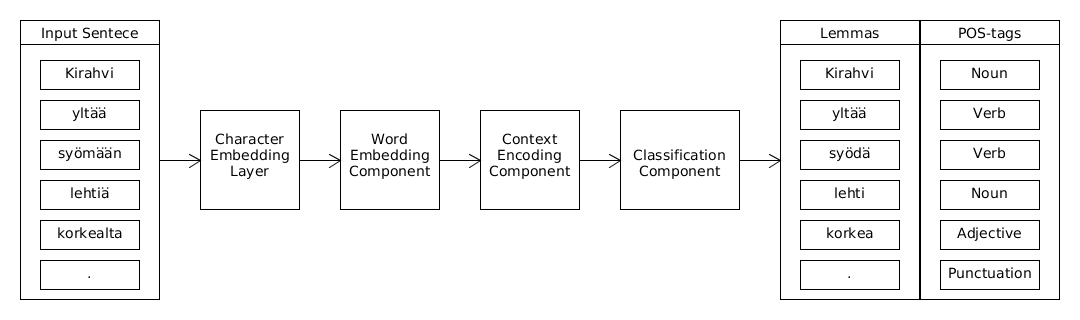
\includegraphics[width=15cm]{architecture.png}
\end{figure}

Neural network code was implemented with Python using popular computation libraries Tensorflow and Numpy. Tensorflow provides scripting APIs for other programming languages too but Python was selected because of it is fast to write and computational performance does not suffer compared to eg. C++ since all the expensive computations are made in the C++ based backend. Numpy is used in the data pre-processing phase where data is processed to be suitable for feeding as input to the actual neural network. Tensorflow was used for implementing the neural network as a computational graph. Tensorflow makes it fairly easy to implement compled multi-componen end to end architectures while abstracting the actual optimization work away from the developer.

Tensorflow also provides a layer of abstraction to execute the computational graph on either CPU or GPU. GPU computations for pleasantly parallel problems such as neural network optimization are significantly faster. Doing the network training and especially hyper-arameter optimization only on CPU would have not been feasible with the hardware resources available. If computations would have been forced to be ran on CPU, there would have not been enough resources to run sufficient number of hyper-parameter optimization runs. Neural network results are often very sensitive to having suitable hyper-parameters and therefore results obtained in the experiments in the worst case could have been unable to provide answer for the hypothesis.

\subsection{Lemmatizations as Classification Only Task}
Approach for lemmatization in this thesis is classification only. POS-tags are a limited set of 31 labels as defined in the Universal Dependencies project but such is not the case for lemmas. When classifying lemmas with neural network one needs an indexed vocabulary of all possible output labels. Having fixed and limited set of lemmas proves to be a challenge for lemmatization.

As discussed earlier the Finnish language suffers from vocabulary explosion even when considering only lemmas and omitting the inflections because Finnish language makes it possible to form compound words very freely. The number of possible combinations created by selecting two or more words for a compound word is way too large to be handled with a linear vocabulary. The word2vec vocabulary which is created from Finnish Internet Parse bank \todo{citation} contains over 1,7 million unique lemmas. Learning to classify this number of lemmas with a corpus of 160 and some thousand tokens is obviously impossible task.

To circumvent the vocabulary explosion problem for output vocabulary fixed and limited set of lemmas were selected from the training set. Selected lemma vocabulary contains 90\% of the use cases in the Finnish Universal Dependencies 1.4 training dataset. The 90\% coverage is formed by selecting the most frequent words only. This lemma vocabulary contains less than nine thousand unique lemmas opposed to over 1,7 million in the word2vec vocabulary. All the lemmas that were left out of the selected vocabulary are treated as unknown tokens meaning that when classifying out of vocabulary lemma the neural network with output an unknown token "<UNK>". Since vocabulary covers 90\% of the uses in training set, 10\% of uses are left out making unknown token a most frequent label.

Having unknown tokens provides it's own set of challenges for downstream processing tasks: information that is supposed to be provided by the lemma is lost with unknown token. One approach for outputting all possible lemmas is to use a generative model such as encoder-decoder model popular in recent studies \todo{citation} for machine translation. Generative model does not classify indices to a fixed vocabulary but generates the lemma one character at a time.

Generative model does solve the problem with lemma vocabulary but introduces a myriad of other problems. Some of the most prominent problems being vastly increased architectural complexity and significantly increased computational complexity and memory requriements. Introducing a encoder-decoder model also introduces problems with observation metrics. POS-tagging and lemma classification are word level prediction tasks and are as such measured with word level metrics eg. accuracy or F1 score. However encoder-decoder model is a character level model which is also observed on character level. Mixing word level classifications and character level classifications fuzzies the meaning of used metrics for evaluation of network performance.

Because of the forementioned problems, the encoder-decoder model was not a part of the implementation used for this thesis and lemmatization is treated as a classification only task. Also it's worth noting that observing lemma classification with POS-tagging should prove to be sufficient for proving or disproving the hypothesis. 

\subsection{Word Embedding Component}
\label{ss:word_embedding_component}
Representing words with multi-dimensional real number vectors is required to encode semantic and syntactic meaning of the words in a way a neural network can understand them as is discussed in section \ref{se:word_embeddings}. Vector representations are created in this work at the same time as neural network is trained to classify lemmas and part of speeches. In other words no external word embeddings are used such as word2vec. Word embedding in this architecture is managed with character to word encoder similar to \cite{Ling2015}.

Word embedding process starts with representing characters as multi-dimensional real number vectors, called character embedding for the rest of this work. Character embeddings as a part of character to word encoder are also trained at the same time with rest of the network. Character embeddings are implemented as a single trainable Tensorflow variable, a two dimensional array where each row contains embedding vector for a single character in the character vocabulary. Character vocabulary is a fixed set of characters selected to represent majority of use cases in currently processed language, Finnish in this case.

\todo{Format this}
\verb£ !"#$%&'()*+,-./0123456789:;<=>?@ABCDEFGHIJKLMNOPQRSTUVWXYZ£ 
\verb£[\]^_`abcdefghijklmnopqrstuvwxyz{|}~ÄÅÖäåö€£

was selected as character vocabulary to be used. This contains ASCII characters from index 32 to index 127 ie. all but ASCII control characters as well as lower and upper case scandic letters used in Finnish and an euro sign €. This character vocabulary covers 99,933\% of character usages in Finnish internet parsebank. A fairly good representation for Finnish language with very reasonable vocabulary size of 103 characters. Characters not included in the selected character vocabulary were substituted with ASCII control character SUB which was added to character vocabulary. Character vocabulary also contained another ASCII control character ETX, which was used for padding all other words to length of longest word in the current mini-batch (Tensors are essentially arrays and as such do not tolerate variable lengths within a single dimension).

Words as input to word vector encoder are represented as Tensors of character embeddings, each row of a single input word contains character embedding for a single character in the word. Input words for the word vector encoder contain character embeddings for all characters in all words in all sentences selected for the mini-batch. If mini-batch size is selected to be 25, then word vector encoder input contains all characters and words for the selected 25 sentences.

\begin{table}[htbp]
\caption{Example input for Word vector encoder}
\label{table:word_vector_encoder_input}
\centering
\begin{tabular}{|r|c|c|c|c|l|}
  \hline
  & $d_0$ & $d_1$ & ... & $d_{299}$ & \\
  \hline
  K & 0.43 & 0.05 & & 0.37 & $t_0$ \\
  i & 0.32 & 0.62 & & 0.80 & $t_1$ \\
  r & 0.45 & 0.69 & & 0.62 & $t_2$ \\
  a & 0.75 & 0.64 & ... & 0.01 & $t_3$ \\
  h & 0.24 & 0.93 & & 0.53 & $t_4$ \\
  v & 0.23 & 0.24 & & 0.15 & $t_5$ \\
  i & 0.32 & 0.62 & & 0.80 & $t_1$ \\
  \hline
\end{tabular}
\end{table}
Table \ref{table:word_vector_encoder_input} shows an example input to word vector encoder RNN with values rounded to two decimals. $d_0$ to $d_{299}$ are the dimensionalities of character embedding vectors and $t_0$ to $t_6$ are RNN input timesteps ie. characters of the word \textbf{\textit{Kirahvi}}. Example provided shows only a single word, in practice the input data contains multiple words all stacked into a single Tensor.

Word vector encoder itself is a bi-directional recurrent neural network which takes the words represented by character embeddings as input and produces word embedding Tensor as output. Characters of the input words are the timesteps data for the RNN. Bi-directional RNN goes through the input timesteps in both directions. Each direction has a single RNN cell and outputs of both cells are concatenated as one double sized Tensor. Word embedding Tensor ie. output Tensor contains a single word embedding on each row. These word embeddings produced by the word vector encoder contain the semantic and syntactic meanings that were obtained from reading the words as separate units without any context.

\begin{table}[htbp]
\caption{Example output of Word vector encoder}
\label{table:word_vector_encoder_output}
\centering
\begin{tabular}{|c|c|c|c|}
  \hline
  $d_0$ & $d_1$ & ... & $d_{299}$ \\
  \hline
  0.96 & 0.12 & ... & 0.87 \\
  \hline
\end{tabular}
\end{table}
Table \ref{table:word_vector_encoder_output} shows an example output of word vector encoder RNN with values rounded to 2 decimals. $d_0$ to $d_{299}$ are the dimensionalities of word embedding vector for a word \textbf{\textit{Kirahvi}}. Example provided shows only a single word, in practice the output data would have several words in a single Tensor, one per row.


\subsection{Context Encoding Component}
\label{ss:context_encoding_component}
Word embedding vectors created with the word embedding components are the foundation for doing word level predictions. Using encoded information about semantic and syntactic information of the words for which predictions are to be made is far superior to simply using eg. one hot encoding as is discussed in section \ref{se:word_embeddings}. However word embeddings are not nearly perfect representation of all the information that is associated with the words because words represented this way are still only separate units without context in which they appear.

More information about words for doing predictions can be gained by encoding the context of the word into a vector representation to be used along with word embedding. Words are read from left to right in most languages forming a sequence, a sentence, in similar way as character sequences form words. Since words in a sentence are sequence, the context of a word is also a sequence. Sequence of a word in this work means word's preceeding succeeding words ie. words on the left and right side of the current word. Because context is a sequence, once again recurrent neural networks are a natural way to process the sequences.

Word's context can be divided into two parts: left side context, the preceeding words, and right side context, succeeding words. To encode both contexts the architecture uses bi-directional RNN. First cell is used process the left side context and second cell is used to process right side context. One could argue that using two bi-directional RNNs, one for each side, would yield better results. However since importance of word in a context is higher closer the contextual word is to current word and since RNNs "remember" the last timesteps the best, it was hypothesised that using only a single direction for each side would yield almost similar results. Sequence direction of a context is always towards the current word, from left to right for left side context and from right to left for right side context making the closest words always last in the context sequences.

Using only a single uni-directional cell for each side also has significant benefits in terms of implementational simplicity and computational complexity. If one were to use bi-directional RNN for each side, one would be forced to run contexts for each word in a sentence separately because in this scenario the backward passes start from different location, from the current word. When using only an uni-directional RNN for each side there are no backward passes and forward passes always start from the same location: first word of a sentence for left side context and last word of a sentence for right side context. Figure \ref{figure:uni_vs_bi} illustrates this difference between uni-directional and bi-directional context encoders. Using uni-directional context encoders makes it possible to do a single forward pass and a single backward pass for entire sentence. Contexts of different words are simply different timestep outputs of these passes.

\begin{figure}[htbp]
\caption{Uni-directional vs bi-directional RNNs for context encoding}
\label{figure:uni_vs_bi}
\centering
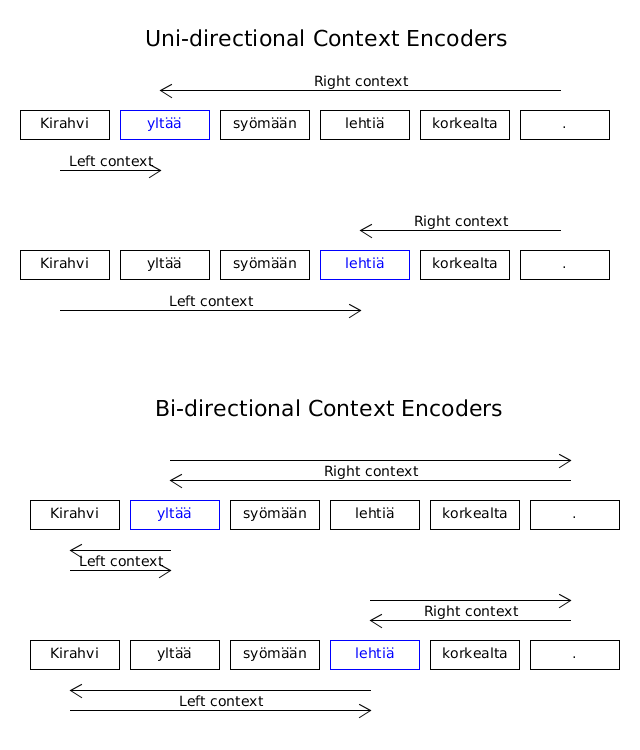
\includegraphics[width=15cm]{uni_vs_bi.png}
\end{figure}

Sharing context encoder passes among all the words in the sentence simplifies input data format of context encoder. Instead of having separate Tensor for each word as input data as is the case with bi-directional RNN, uni-directional can use a single Tensor which has all the words stacked, one word embedding vector per row. Having one simple input Tensor entails a single data pass through the RNN decreasing computational complexity drastically. For a 13 word sentence one would have to make 14 passes for left side (1 forward, 13 backward) and another 14 passes for right side if one were using bi-directional RNN. With uni-directional RNN this comes down to one pass per side, 14 fold decrease. Actual computation time decrease might smaller because it could be possible to parallelize this operation with GPU. Measuring actual prediction performance benefits and added computational costs associated with using bi-directional RNN for context encoder is out of scope for this thesis. Table \ref{table:context_encoder_input} shows an example of input data Tensor for context encoder when using batch size of one sentence. $d_0$ to $d_{299}$ are dimensionalities of word embedding vectors.
\begin{table}[htbp]
\caption{Example input of context encoder}
\label{table:context_encoder_input}
\centering
\begin{tabular}{|r|c|c|c|c|l|}
  \hline
  & $d_0$ & $d_1$ & ... & $d_{299}$ & \\
  \hline
  Kirahvi & 0.96 & 0.12 & & 0.87 & $t_0$ \\
  yltää & 0.16 & 0.26 & & 0.65 & $t_1$ \\
  syömään & 0.24 & 0.51 & & 0.80 & $t_2$ \\
  lehtiä & 0.05 & 0.55 & ... & 0.96 & $t_3$ \\
  korkealta & 0.82 & 0.06 & & 0.39 & $t_4$ \\
  . & 0.03 & 0.14 & & 0.46 & $t_5$ \\
  \hline
\end{tabular}
\end{table}

Context encoder RNN produces embedding vectors of a similar form as is it's input ie. output of word embedding component. These vectors encode semantic, and some syntactic, meaning of the words' contexts. When used with word embedding vectors these two encodings express all the information that is available for the words when looking only at the sentence. Output of the context encoding component is vector formed by concatenating word embedding vectors and context embedding vectors for respective words. Table \ref{table:context_encoding_component_output} shows an example output for a single word from context encoding component. $d_0$ to $d_{299}$ are dimensionalities of word embedding vectors and $d{300}$ to $d_{599}$ are dimensionalities of context encoding RNN.
\begin{table}[htbp]
\caption{Example output of context encoding component}
\label{table:context_encoding_component_output}
\centering
\begin{tabular}{|r|c|c|c|c|c|c|c|c|l|}
  \hline
  & $d_0$ & $d_1$ & ... & $d_{299}$ & $d_{300}$ & $d_{301}$ & ... & $d_{599}$ & \\
  \hline
  Kirahvi & 0.96 & 0.12 & & 0.87 & 0.69 & 0.88 & ... & 0.74 & $t_0$ \\
  \hline
\end{tabular}
\end{table}

Higher level contructs for information encoding, such as looking at preceeding and succeeding sentences in the corpus, are not used in this architecture. Adding contextual information for sentences would add yet another layer of complexity to the architecture increasing actual implementational difficulty significantly. Reshaping Tensors in Tensorflow can be very tricky at times, especially when splicing and stacking for batching has to be done on multiple architectural levels. Also using sentences' contexts could prove problematic when using the neural network for actual live production work because it is often the case that user wants lemmatization and POS-tagging done for a single sentence without having context at hand.


\subsection{Classification Component}
\label{ss:classification_component}
Output of context encoding component could very well be used for doing predictions given that output is projected to a suitable size, namely the number of classes to classify. However architecture used in this work has additional fully connected layers between the output projection layer and context encoding component. In this configuration the architecture can be divided into two logical sections: encoder and classifier. Figure \ref{figure:encoder_classifier} shows the two logical high level components of the architecture.

\begin{figure}[htbp]
\caption{High level logical components of the architecture}
\label{figure:encoder_classifier}
\centering
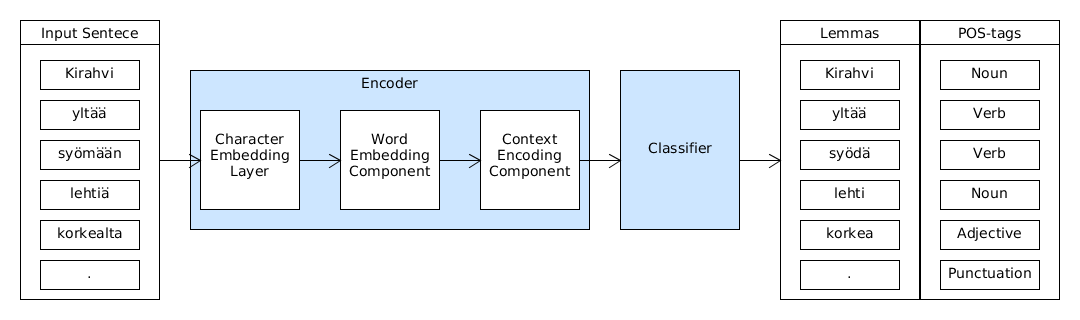
\includegraphics[width=15cm]{encoder_classifier.png}
\end{figure}

Encoder composes of all the layers and components up to the classification component and the classifier is a simple fully connected feed-forward network, also called multi-layer perceptron (MLP). When conseptualized in this way, the responsibility of the encoder is to, as name suggest, encode all available input information in a format which is easily understood by the classifier. Classifier is responsible to produce the actual predictions. Input of the classifier is the output of the encoder as is, without any projections or scaling. When the architecture is build by separating the encoder and the classifier, it is easier in the future works to reuse the encoder and create a new classifier suitable for the task at hand. On the other hand the classification component can be thought to be just a few fully connected layers on top of context encoding component for added expression power.

Regardless of how one wishes to approach the logical components of the architecture, the fact remains that the fully connected layers were added based on early experiments on the architecture's learning capabilities. With few training runs on different configurations it became clear that neural net converges to a better performing model when using the fully connected layers than without them. Without the fully connected layers the network seemed to converge faster, with less epochs, but couldn't obtain quite as high classification performance. It is also worth mentioning that adding even several fully connected layers added almost no extra computational cost. Multiple layers of RNNs seem to be a lot more expensive than even far greater number of fully connected layers.

The last two layers of the classification component are output projection layer and softmax layer. The output projection layer is fully connected layer with linear activation function and has one node for each class. The softmax layer takes the output of projection layer can computes a softmax function for it, this is done to scale the output values in such a way that all output values sum up to one. When outputs are scaled to sum up to one, the output can be treated as probability distribution even though it might not strictly be one. Scaled outputs are also easier for humans to understand, often a nice to have feature but certainly not critical. The main reason to add a softmax layer after the output prediction really lies with the softmaxes innate properties which make it suitable for optimization with cross entropy loss.

As a matter of fact the softmax layer only exists in the training pipeline. Softmax scaling is not necessary for doing the predictions because the prediction of a classifier is the output node with highest activation value. Softmax is a monotonic function ie. higher input values will always give higher output values and since the classification is only about selecting the highest value, the softmax is not required. In addition the softmax can be computationally relatively expensive especially when the output size is large, as is the case with large lemma vocabulary.

To produce the actual lemmas and part of speeches, the indices of the highest values in the output layer need to be used for indexing the label vocabularies. If the third node on the lemma output layer has highest value, one must select third item in the lemma vocabulary as the final prediction. Vocabularies are not needed for testing and validating because the ground truth lemmas and part of speeches have also been turned into indices and comparison can be done with the indices.

\subsection{Training and Optimization}
All neural network trainings in this work were done with stochastic gradient descent back-propagation algorigthm. The optmizer algorithm and back-propagation through the computation graphs are handled by Tensorflow's built in features. First the input data is fed to neural network and propagated in forward direction through the whole network. When the last network layer, the softmax layer, has been computed, the softmax values are used to compute cross entropy loss with one-hot coded ground truth vector. Error gradient is then propagated through the entire network in backward direction, calculating error gradient for each layer. Error gradient in each layer is used to update the layer weights and biases.

Gradient descent update was done with mini-batches of 25 sentences. This means that entire mini-batch is back-propagated through the network before adjusting the network weights and biases. Alternative is to update the network after each example but that has serious drawbacks for computational efficiency. Mini-batch training can be done in a pleasantly parallel manner, meaning that the exapmles of the mini-batch have no cross-dependencies and thus can be all trained at the same time, parallel. Parallel computations are very suitable for GPU workloads and as a matter of fact mini-batch training is critical component for enabling the significant, often an order of magnitude or more, increases in computation speed on GPU. Figure \ref{figure:single_vs_batch} illustrates the difference between the propagation sequences in single example training and mini-batch training.

\begin{figure}[htbp]
\caption{Propagation sequences in single exmaple and mini-batch training}
\label{figure:single_vs_batch}
\centering
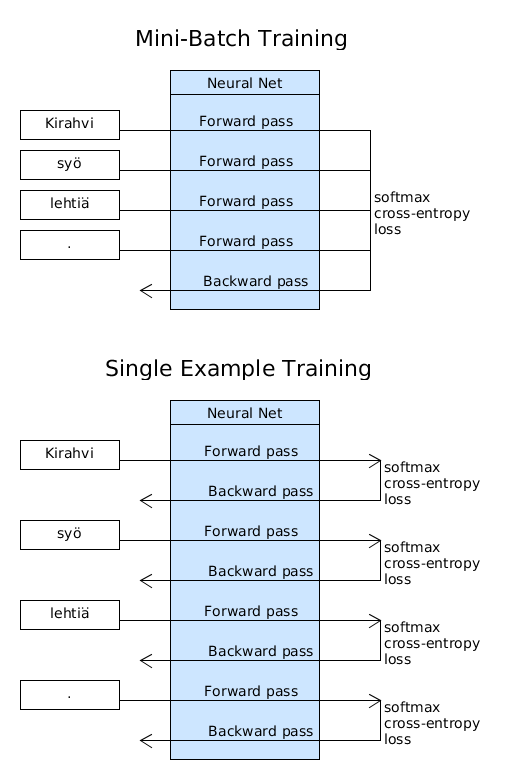
\includegraphics[width=12cm]{single_vs_batch.png}
\end{figure}

Also a true single example training is not even possible, at minimum a mini-batch contains all the words of a single sentence. The reasons for this are the facts that the single example of input-output value pair is a single word and it's lemma of POS-tag and a word depends on it's context ie. other words in the sentence. Therefore it's mandatory to use at least a single sentence mini-batching. If architecture didn't contain the context encoding component, all words of the sentence could be managed as separate units and could be trained independently.

Mini-batches of 25 sentences used for network optimization are formed by dividing the entire training dataset randomly into the said mini-batches. Training procedure goes through all the mini-batches in an epoch. In the end of the epoch after all of the training data has been used, the network classification performance is evaluated on the validation dataset by calculating loss. Loss is the compared to the best obtained loss value from all the previous epochs, if the validation loss has decreased training procedure continues onto the next epoch. If validation loss doesn't decrease training can be stopped to avoid over-fitting. However classification performance on validation dataset does not typically improve on every epoch, especially after the network is starting to converge. Therefore it's wise to allow the training to continue for a fixed number of epochs even if there is no improvement. When the maximum number of epochs without improvement has been reached, the training is stopped and classification performance is tested on the testing dataset.

The network training procedure described above is only a single training run. Single training run allows the optimization of network parameters (weights and biases) but not hyperparameters. Hyperparameters are all the parameters that determine the network architecture, such as number of layers on each component, number of nodes on each layer, activation functions used, dropout etc. Traditionally hyperparameters have been optimized by manual process of training with certain cofiguration, inspecting the results, adjusting hyperparameters and training again. While manual hyperparameter optimization can provide good enough results, it is still very tedious work and often requires deep understanding of neural networks and of the task at hand. Recently automatic hyperparameter optimization has gained popularity, mainly because computation resources have increased and thus it's more feasible to run a lot of training runs while tuning the hyperparameters. Automatic hyperparameter tuning is particularly beneficial when the number of hyperparameters to optmize gets large, humans are typically poor at processing more than 3 dimensional data.

Hyperparameter optimization in this work was done automatically using a optimization library called Optunity \todo{citation}. Optunity provides a convenient way to abstract the optimization work for basically any given task. There are many different optimization algorithms for hyperparameter tuning and not one has gained similar de facto status as gradient descent has for the neural net optimization. Algorithm used in this work for hyperparameter tuning is particle swarm which is a meta heuristic optimization algorithm. Particle swarm is said by the Optunity authors to be most versatile of all the algorithms available in Optunity. Hyperparameter optimization algorithm comparisons were not done since particle swarm provided reasonable results with the time results of this project. Besides hyperparameter optimization algorithm selection is not in the scope of this work and has very little relevance with proving the hypothesis.

Hyperparameter optimization was done by running a fixed number of training runs and tuning the hyperparameters with particle swarm between each training run. Since automatic hyperparameter selection may ramp up all the hyperparameters to their maximum allowed values, can training times scale up to unsustainable durations. To avoid dealing with single training runs that take tens of hours, maximum time budget was forced for the training runs. If training run reached the maximum allowed time, best model obtained with that training run was selected for final comparison and hyperparameter tuning. Training runs in the hyperparameter optimization also used early stopping based on validation loss, this helps to cut the training with some hyperparameter configurations to just few training epochs, speeding up the hyperparameter optimization drastically.

After all of the training runs for hyperparameter optimization were finished, hyperparameter configuration which provided the best model was saved for using in experiments.

\section{Experiments}
\label{se:experiments}
Experiments done for this thesis consist of minimal set of tests that can prove or disprove the tested hypothesis. To test whether jointly learning lemmatization and POS-tagging in a single neural network architecture the following experiments were done. Firstly a baseline was established by training and testing the neural net with lemmatization and POS-tagging as separate tasks. Having a well established baseline allows the comparison of different style shared information tasks and their benefits and drawbacks. Figure \ref{figure:baseline_experiment} shows the setup for separate tasks.

\begin{figure}[htbp]
\caption{Separate lemmatization and POS-tagging as a baseline}
\label{figure:baseline_experiment}
\centering
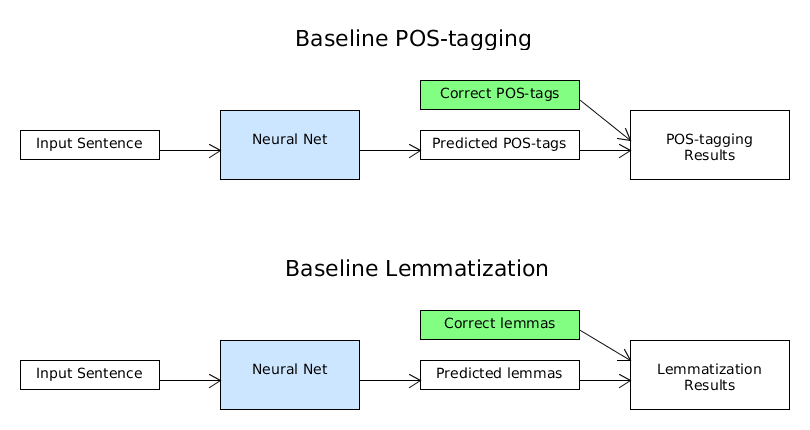
\includegraphics[width=15cm]{baseline_experiment.png}
\end{figure}

First shared information experiment was done to determine if more traditional approach of using one as input features in classification of other. This experiment was done only by using parts of speech as one-hot coded input features when doing lemma classification. Expecting to gain benefit from using parts of speech as input feature to lemmatization is reasonably well founded because knowing the part of speech for a given word limits the number of possible lemmas significantly. The big question in this hypothesis is whether the POS-tagging was done well enough to reveal the possible benefits. It's very well possible that errors done in POS-tagging cascade to lemmatization task so badly that lemmatization performance actually decreases from the baseline. To study the effects of POS-tagging performance to lemmatization performance, a second experiment was deviced: to train and test the network using gold-standard parts of speech available in the dataset. Figure \ref{figure:pos_tag_input_experiment} shows the setup for using parts of speech as input feature for lemmatization.

\begin{figure}[htbp]
\caption{Using parts of speech as input feature for lemmatization}
\label{figure:pos_tag_input_experiment}
\centering
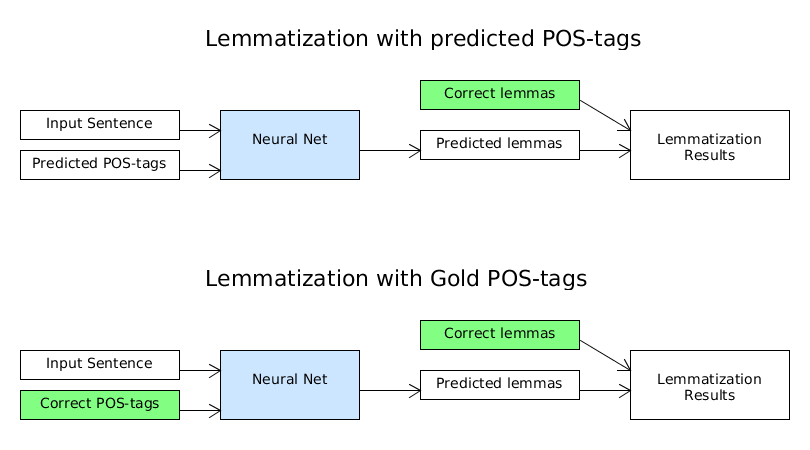
\includegraphics[width=15cm]{pos_tag_input_experiment.png}
\end{figure}

Last experiment was the training and testing of the joint learning neural network architecture for lemmatization and POS-tagging. Figure \ref{figure:joint_model_experiment} illustrates the test setup for joint model.

\begin{figure}[htbp]
\caption{Joint model for lemmatization and POS-tagging}
\label{figure:joint_model_experiment}
\centering
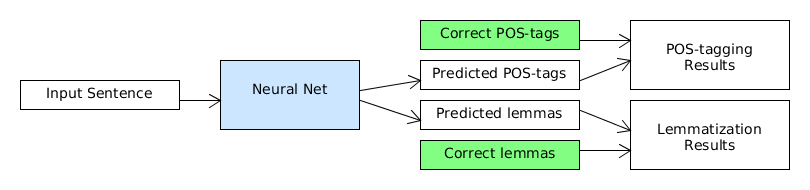
\includegraphics[width=15cm]{joint_model_experiment.png}
\end{figure}

Comparing results from the baseline, POS-tags as input features for lemmatization and joint model should be enough to test the hypothesis. Experiments don't include other languages than Finnish or other datasets than Finnish Universal Dependencies. Experiments in this thesis with POS-tagging all use the universal POS-tags, effect of using language specific POS-tags with or without universal POS-tags was not tested. Similarly effect of tokenization performance was not tested but all experiments used gold standard tokenization available in the Finnish universal dependencies dataset.

The effect of morphological information such as word inflections and forms were not tested for this thesis even though there is a well founded arguments for improving results by using the morphology also. Since morphological features describe how the word was inflected they should assist the lemmatization because lemmatization can though as a reverse process of inflecting the word. However scope of the thesis was kept as narrow as possible, but wide enough for testing the hypothesis, and therefore morphology was left out. For that same reason also use of language specific POS-tags available in Universal Dependecies datasets was left out of scope of this thesis. 

Attentive reader might have noticed that experiments included in this thesis have parts of speech as input features for lemmatization but not lemmas as input features for POS-tagging. Reason for excluding experiment of lemmas as input features for POS-tagging is that the described task is not very interesting or even meaningful: if a lemma of a word is known, part of speech for that word can be looked up from a dictionary with the exceptions of words with multiple meanings.


\section{Test Methods}
\label{se:test_methods}
\todo{Excerpt from Finnish UD data}
\begin{itemize}
\item Testing with Universal Dependencies data
\item Finnish UD data is tagged with Omorfi and manually corrected, see \ref{ss:turku_dependency_treebank} \todo{Check manual correction}
\item UD has pre-existing results from third parties such as Syntaxnet and UDPipe for baseline comparisons
\item Other annotated corpuses exist for Finnish but UD is the only multi-lingual corpus collection where all datasets are in uniform format making future research and comparison easier. \todo{citations!}
\item Using accuracy. Percentage of correct classification labels.
\item Academia does not seem to agree what F1 score is
\item Accuracy is simple and easier for the readers to understand
\item Accuracy may not be suitable if neural network prediction confidences are important. Neural net may learn to be very confident about wrong predictions if only accuracy is observed.
\item Accuracy is suitable to distinguish between results on different configurations. Confidences are not needed for this work.
\item Cross-entropy based loss is good for weight optimization and does not suffer from confidence issues but tells very little to a reader without deep understanding about the task at hand.
\item Each experiement was executed by training the network on the training dataset with early stopping based on observations of validation dataset loss.
\item Same hyperparameters were used for all experiements, tuned with Optunity implemented particle swarm algorithm for joint model.
\item All results reported are tested with test dataset.
\item Tokenized data (forms) is fed to neural network as input and neural network predictions are compared to correct values.
\end{itemize}

\section{Results}
\label{se:results}
\begin{itemize}
\item UDPipe 1.2 achieves 94,9\% on POS-tagging on Finnish Universal Dependencies 2.0 and 86,8\% on lemmatization. Both results with gold tokenization. \cite{udpipe-manual}
\item UDPipe lemmatizer is a generative model (\cite{Straka2017}), so comparison is not fair or even meaningful.
\item POS-tagging without lemmatization = 94,30\%. Remarkably close to UDPipe results with only 0,6\%-points advantage to UDPipe. Limited mainly by data?
\item Lemmatization without POS-tagging = 94,25\%
\item Lemmatization with classified POS-tags as input features = 94,40\%
\item Lemmatization with gold standard POS-tags as input features = 96,22\%
\item Joint model. Lemmas = 95,24\%, POS = 94,14\%
\item Joint model achieves best practical results for lemmatization, with 0,99\%-points increase, since gold-standard POS-tags are not available for live inferencing.
\item Joint model POS-tags are slightly inferior (0,16\%-points) to baseline
\item Lemmatization results with classified POS-tags are slightly better (0,15\%-points) than the baseline.
\item Lemmatization with gold-standard POS-tags achieves clearly the best results with 1,97\%-points increase over baseline.
\end{itemize}


\chapter{Discussion}
\label{ch:discussion}
\section{How well results generalize?}
\begin{itemize}
\item Do these results generalize to other languages needs to be verified with additional experiments.
\item Universal Dependencies datasets are created to provide as uniform language modeling as possible across all languages and therefore it is probable that the same mutual information between lemmas and POS-tags in other languages would prove beneficial in joint learning of lemma and POS-tag classification.
\item Speculating how well these results generalize to other tasks in natural language processing is more complicated because other tasks may not share as strong mutual information as lemmas and POS-tags do.
\item \cite{Liang2016a} proved that neural networks benefit from jointly learning two tasks different from lemmatization and POS-tagging. \cite{Liu2016a} even had tasks on different architectural level, slot filling being word level task and intent classification being sentence or message level task.
\item With results provided in this work and results from \cite{Liu2016a} it's failry safe to say that neural networks can obtain better results when learning jointly two tasks that share mutual information.
\end{itemize}

\section{What was assumed?}
\begin{itemize}
\item It was assumed that training dataset would represent Finnish language well. May not hold true since all sources of the dataset are from internet.
\item It was also assumed that different datasets would have fairly similar data distribution and training done on training dataset would generalize to test dataset.
\item It was noticed that selecting lemma vocabulary which covers 100\% of uses in training set only covers about 75\% of uses in validation and test datasets.
\item Lemma classifier learned remarkably well to classifiy lemmas not seen during training time as unknown tokens. Maybe priori bias explains this?
\end{itemize}

\section{What was simplified?}
\begin{itemize}
\item Slightly different results would be optained by optimizing hyperparameters separately for every different experiement. Hyperparameter optimization requires about 100 to 200 training runs and as such takes significant time budget. Using time required for hyperparameter optimization before every experiement proved inconvenient for this work.
\item Hyperparamenter optimization do not have variation with loss weights for the two tasks. Loss weight sets the target if optimizing based on validation loss and therefore cannot be optimized.
\item Hyperparameter optimization was using time budget for each run
\item Hyperparameter optimization had limited number of runs available
\item Selecting a different optimization target for hyperparameters could have allowed loss weight optimization.
\item Character vocabualry for C2W does not contain all characters in datasets. Even still embedding vectors for some characters are probably not well learned because of their unfrequency. 
\item Lemmatization as word level classification task only is also a pretty significant simplification. Decoder model for lemma generation is able to always produce some kind of answer without ever producing unknown tokens.
\item Selected lemma vocabulary covers 90\% of the training set -> unknowns are 10\%, second most frequent is less than 5\%. It was not tested if unknown prediction accuracy would break if unknowns weren't the most frequent.
\item Whether having unknown tokens is fatal flaw depends on the problem at hand and on the down stream processing which uses lemmas obtained with lemmatization. For some tasks not having generated lemmas with high probability of typographical errors produced might be significantly better option.
\item Experiements done with golds standard tokenization of Universal Dependencies datasets. In live production such tokenization is not available. Imperfect tokenization may completely ruin the classification if tokens are not created correctly.
\item Same applies for sentence segmentation.
\end{itemize}


\chapter{Conclusions}
\label{ch:conclusions}
\begin{itemize}
\item Hypothesis proved to be true, at least partly
\item Neural networks are very suitable for joint learning tasks.
\item Uncorrelated tasks are not tested yet but those don't have any obvious theoretical foundation why they should benefit.
\item Interestingly we couldn't obtain increase in POS-tagging performance.
\item Maybe lemmatization as a more information rich task dominates the learning
\item POS-tagging on joint model could be improved by giving more weight to POS-tagging task but that quickly deteriorates the lemmatization perfomance drastically.
\item Doing neural net based lemmatization benefits from jointly learning also to POS-tag. Added architectural, implementational and computational complexities are minor.
\item Author recommends always to do POS-tagging when doing lemmatization.
\item If main task is POS-tagging, adding lemmatization is probably not beneficial enough for the added computational cost.
\item If both tasks need to be done and POS-tagging performance is a priority it might prove to be difficult to achieve best possible results with joint model.
\end{itemize}

%
% The bibliography, i.e the list of references (3 options available)
%
\newpage


% Extra for Finnish theses

\renewcommand{\bibname}{Bibliography}     % Bilingual babel puts Finnish ``Kirjallisuttaa'' otherwise. Strange...
%\renewcommand{\bibname}{Lähteet}         % Set Finnish header, remove this if using English
%\addcontentsline{toc}{chapter}{Lähteet}  % Include this in TOC
\addcontentsline{toc}{chapter}{\bibname}  % Include this in TOC


\printbibliography                  % a) heading in English
%\printbibliography[title=Lähteet]   % b) heading in Finnish
%\addtocontents{toc}{%               % b) add Finnish heading to table of contents
%\protect\noindent Lähteet\protect\par
%} 


%
% Appendices are optional. 
% This part is semi-ugly at the moment. Please give feedback if can
% improve it.
\appendix
\pagestyle{headings}
% \renewcommand{\appendixname}{Liite} % Extra. Set Finnish prefix for page header

%
% a) Not-so-handy way, but at least it works
% 
\def\appA{APPENDIX A. Something extra} % Define the name and numbering manually
\chapter*{\appA}                       % Create chapter heading
\markboth{\appA}{\appA}                % Set page header
\addcontentsline{toc}{chapter}{\appA}  % Include this in TOC
% Note that \label does not work with unnumbered chapter

Appendices are purely optional.  All appendices must be referred to in
the body text

\def\appB{APPENDIX B. Something completely different} % Define another new command
\chapter*{\appB}                       % As above, but use \appB instead of \appA
\label{app:B}
\markboth{\appB}{\appB}                     
\addcontentsline{toc}{chapter}{\appB}  


You can append to your thesis, for example, lengthy mathematical
derivations, an important algorithm in a programming language, input
and output listings, an extract of a standard relating to your thesis,
a user manual, empirical knowledge produced while preparing the
thesis, the results of a survey, lists, pictures, drawings, maps,
complex charts (conceptual schema, circuit diagrams, structure charts)
and so on.


%
% b) The other option is to use numbered chapter and our baseline
% template report.cls numbers them as A, B... The heading and TOC do
% not include prefix 'Appendix' although the page header does.
%\chapter{name of the appendix}
%\label{app:A}                          % For cross-references



\end{document}

